% normal report style
\documentclass[11pt, a4paper]{report}

% thesis details
% ---------------------------------------------------------------------------
\newcommand{\submissionDate}{9. June 2016}
\newcommand{\titleFirst}{Historical Geographic Information Systems --}
\newcommand{\titleSecond}{Modelling Changes in Time and Space}
% ---------------------------------------------------------------------------

%\*** INCLUDING PACKAGES ***\
\usepackage[utf8]{inputenc}     % encoding in UTF-8
\usepackage{lmodern}            % makes pretty font
\usepackage{amsmath}            % math mode with $ $
\usepackage{amssymb}            % several math symbols
\usepackage{textgreek}          % for Greek letters
\usepackage{cite}               % numerical citation
\usepackage{url}                % url mode for bibtex
\usepackage{graphicx}           % includegraphics
\usepackage{moreverb}           % for verbatimtab
\usepackage{fancyhdr}           % customise the page header
\usepackage{array}              % for removing vertical space of lists inside tabulars
\usepackage{enumitem}           % allow itemsep in list environments
\usepackage{supertabular}       % for tabular with page break
\usepackage{wrapfig}            % for floating text around images
\usepackage{geometry}           % set page margins manually
\usepackage{float}              % for positioning options for containers h!
\usepackage{pdfpages}           % include foreign pdf files
\usepackage{hyperref}           % cliackable toc
\usepackage{titletoc}           % manipulate toc
\usepackage{caption}            % to center captions figures
\usepackage[super]{nth}         % for 1st, 2nd, 3rd, ...
\usepackage{textcomp}           % gets rid of gensymb (v) package warning
\usepackage{gensymb}            % for ° symbol
\usepackage{alltt}              % allows symbols in something like verbatim
\usepackage{subcaption}         % allows multiple graphics per figure
\usepackage{booktabs}           % for fancy tables
\usepackage{multirow}           % for merging cells on multiple rows


%\*** HYPHENATION RULES ***\
\hyphenation{Haupt-schule}


%\*** FORMAT & STYLE ***\

% page margins
%\geometry{a4paper, top=25mm, left=30mm, right=30mm, bottom=30mm, headsep=10mm, footskip=12mm}

% set Helvetica (like Arial) as standard font for the document
\renewcommand{\familydefault}{\sfdefault}

% line spacing
\linespread{1.2}

% distance between footnotes and text
\setlength{\skip\footins}{20pt}

% set space to new paragraph, but no indent
\setlength{\fboxsep}{0pt}
\parskip 11pt plus 1pt minus 1pt
\parindent 0pt

% header-left: section name, header-right: nothing, bottom-center: page numbers
%\setlength{\headheight}{15.2pt} % latex hack that prevents error message
%\pagestyle{fancy}
%\rhead{\HG}

% make quotes italic
\newenvironment{quoteit}
{\begin{quote}\itshape}
{\end{quote}}


%\*** NUMBERING AND TOC ***\

% start with sections
\renewcommand{\thesection}{\arabic{section}}

% numbering of subsubsections
\setcounter{secnumdepth}{3}

% include sections -> subsections -> subsubsections in toc
\setcounter{tocdepth}{3}

% configure toc            left indent space up/down      font              position of numbers        filling until        page number
\titlecontents{section}       [3.7em]  {\addvspace{+0.2em}\large\bfseries} {\contentslabel{2.2em}} {} {\hfill               \contentspage}
\titlecontents{subsection}    [6.7em]  {\addvspace{-0.6em}\large}          {\contentslabel{2.95em}}{} {\titlerule*[0.6pc]{.}\contentspage}
\titlecontents{subsubsection} [10.6em] {\addvspace{-0.8em}\normalsize}     {\contentslabel{3.8em}} {} {\titlerule*[0.6pc]{.}\contentspage}

% configure clicking on toc
\hypersetup{
    colorlinks,
    citecolor=black,
    filecolor=black,
    linkcolor=black,
    urlcolor=black
}

% some weird hack to get rid of the vertical space in lists inside tabulars
\makeatletter
\newcommand*{\compress}{\@minipagetrue}
\makeatother


% meta information
\title{\titleFirst \\ \titleSecond}
\author{Marcus Kossatz}
\date{\submissionDate}


\begin{document}

%\* TITLE PAGE *\

\begin{titlepage}

Bauhaus-Universität Weimar \\
Faculty of Media \\
Degree Programme Computer Science and Media \\ [2.0cm]

\begin{center}

{\huge \titleFirst} \\[0.5cm]
{\huge \titleSecond} \\[3.5cm]
\end{center}

{\LARGE Master's Thesis} \\[1.0cm]

Marcus Kossatz \hfill Matriculation Number 90487 \\
b. 21.08.1989 in Spremberg, Germany \\

1. First Referee: Univ.-Prof. Dr.-Ing. habil. Volker Rodehorst \\
2. Second Referee: Prof. Dr. rer. nat. Sven Bertel \\

\vfill
Submission date: \submissionDate

\end{titlepage}


%\* LISTINGS *\

\tableofcontents

\listoffigures
\listoftables


%\* DECLARATION *\

\newpage

\section*{Selbstständigkeitserklärung}

\vspace{10px}

Hiermit versichere ich, dass ich die vorliegende Masterarbeit selbstständig und nur unter Zuhilfenahme der angegebenen Quellen erstellt habe.

\vspace{20px}

\hfill \rule{120px}{0.5px} \\
Weimar, \submissionDate \hfill Marcus Kossatz

\newpage


%\* ACKNOLEDGEMENTS *\

%!TEX root = ../masters_thesis.tex

\section*{Acknowledgements} % (fold)
\label{cha:acknowledgements}

Rodehorst
Bertel

UVa Scholar's Lab
Ammon
Purdom
Jeremy
Chris
Wayne
Eric
Scott
Ronda
Laura
Becca
Shane
Veronica

parents

friends

John Oliver Last Weeks Tonight

% chapter acknowledgements (end)



%\* CONTENT *\

%!TEX root = ../thesis.tex

\section{Introduction}
\label{sec:introduction}

\begin{quoteit}
\large
La Géographie n’est autre chose que l’Histoire dans l’espace, \\
de même que l’Histoire est la Géographie dans le temps. \\

Geography is nothing but History in space, \\
the same way as History is Geography over time.
\end{quoteit}
\hfill \textit{-- Élisée Reclus: ``L'Homme et la Terre'' (1908)}

From everything we know by today, our planet Earth is the only place in our universe that is habitable for us. About 200,000 years ago the \emph{homo sapiens sapiens}, the first modern human beings, settled in nowadays Africa. 125,000 years ago humans conquered fire and the advent of agriculture 10,000 years ago started permanent human settlements in villages and introduced the end of nomadic human life. The settlements were often close to natural water, at rivers, lakes or the coast. Water is the most essential element -- and knowing where it is one of the most essential tasks for early human beings. Finding the habitat of animals was crucial for hunters, the location of bushes and shrubs for gatherers. Knowing the closest lookout was helpful to observe herd moving or get the latest weather forecast. Since the early days of mankind, knowing \emph{where} things are was essential for survival or at least helpful in the daily lives.

There is one tool that has been used already in early civilizations -- and it is one of the most beautiful and representative documents of these times: A map. It is a physical expression of something that is not tangible: The structure, the surface, the population of the Earth's surface. The old map that we know of was dates 4,000 years back, to the time of the Akkadian Dynasty of Sargon in Mesopotamia, currently Iraq. Ever since maps became important, may it be for navigators on their explorations on sea, in the field of land-use planning to design our human settlements or for rescue services on their mission to save the lives of people in danger. Nowadays, these tasks are fulfilled using geographic information systems (GIS) -- with a map being their most common type of presentation.

However, most of GIS answer two basic questions about an inspected object: \emph{Where} the object is in relative or absolute location and \emph{what} it is, being its attributes or properties. As an example, a city will have an exact geographic location, expressed in coordinates. Additionally there can be meta-information about the place: Its name, its population or the current rate of unemployment.

%For urban planners there will be certain areas, for example residential, industrial or governmental areas which have different properties based on the different kinds of buildings, their purposes, sizes and prices. For a rescue service it is important to know where their rescue units currently are, which areas have already been searched to reason about to which areas the teams should be tasked to next.

However, most of the GIS that are used nowadays focus mostly on spatial information and are limited to answer these two question. But what about the dimension of time? The answer to the question \emph{when} a city was found, how its population or city borders have developed over the previous fifty years or at what point we can expect it to reach a new threshold of population? To answer these questions, most of the GIS currently in use are not suitable and task-specific systems have to be used. The reason is that the temporal information is not supported most by GIS. But it is exactly the dimension of time that is so strongly related to our lives. It is the core aspect of history -- the study of our past, to understand the present and reason about the future.

Time and space are often tied, just as the French geographer Élisée Reclus described it in his study about human history on Earth. A connection of time and space in an \textbf{Historical geographic information system} \emph{(HGIS)} has a great potential to teach, learn and understand processes in the past. A system that is able to tell \emph{what} happened and \emph{where} the historical event has influences on and \emph{when} the event happened happened might be tool to answer the most important of all questions: \textbf{\emph{Why}} it happened?

This thesis deals exactly with that topic: How can an information system be designed that is able to gather, manage and present historical changes of countries in the course of history? To be more precise, the thesis will deal with the following research questions:

\begin{enumerate}
  \item How to represent the temporal changes of countries, their borders and their names in a geographic information system?
  \item How to visualize these historical changes on the map?
  \item How to deal with uncertainty, imprecision and debated territories?
\end{enumerate}

The work will first lay a foundation with an overview of the working of a GIS and the analysis of existing approaches of spatio-temporal knowledge representation. Afterwards, an own concept to overcome shortcomings of the existent approaches will be developed. This concept will be implemented using \textsc{HistoGlobe}, an existing Web-based visualization of the historical development of countries, which will extent the software to a full HGIS. Finally, the concept will be evaluated in a user study and its implications can be used to determine future work to be done in the field of Historical geographic information systems.

\subsubsection{Motivation} % (fold)
\label{ssub:motivation}

% subsubsection motivation (end)


\subsubsection{History} % (fold)
\label{ssub:history}

% subsubsection history (end)


\subsubsection{Geography} % (fold)
\label{ssub:geography}

% subsubsection geography (end)


\subsubsection{Research Questions} % (fold)
\label{ssub:research_questions}

% subsubsection research_questions (end)


% section introduction (end)


visualizing the course of history on a map and a timeline
-> setting a date on the timeline, seeing the status of history at this point on the map and emphasizing the changes since the last time

status = names and borders of countries
changes = change of names and borders of countries

system already works in browsing mode, i.e. experience history:
http://histoglobe.com
(Europe 1871-1990)

problem: very little data, data entry into the system is horribly complicated, there is no backend

solution: an editor for historical data.

problem: it has to cope with data that is depended on time (how long is the country active?) and space (what is the territorial extent ,i.e. the border, of the country?) -> spatio-temporal data

solution: application of spatio-temporal data models

problem: there are a lot of them

solution: choose the best

problem: there is no ``best''. Each and every one has advantages and disadvantages

solution: alright, then take the one with the biggest advantages.

comparison of two models: snapshot model (SM) vs. event-based spatio-temporal data model (ESTDM)

SM: save the status of the world at time point t_1 (e.g. 1945) and time point t_2 (e.g. 1990)
(+) very easy
(+) concept well known from historical maps
(+) very helpful if the status at the years directly is to be seen (e.g. 1945 or 1990)
(-) what if I want to know how the world looked like at t_x (e.g. 1975)
=> it does not work, because there is no information
(-) every time something changes on the map a total new image would have to be saved
=> very redundant and inefficient

ESTDM: save the status of the world at one reference time point t_r (e.g. 1945) and from there on save only changes to this one, e.g.
1949: separation of Occupied Germany into East Germany and West Germany and ceding of parts of the country to Poland
1990: unification of West Germany and East Germany to Germany
(-) a little bit more complex
(+) for each point in history the status of the world can be retrieved: it is the status at the reference time point t_r and all changes until this point accumulated and applied on the map
(+) historical changes can easily be visualized on the map, because they are stored explicitly
(-) storing a change backwards (e.g. 1933: rename of Weimar Republic into Nazi Germany) is more complex, because it has to be applied in the opposite direction

there are some more problems I dealt with. But finally I have developed a prototype that can do that (click_prototype.pdf) that can do it. This prototype was developed with the aid of the people in Scholar's Lab that have been a big part of my development process.

%!TEX root = ../masters_thesis.tex

\chapter{Basics} % (fold)
\label{cha:basics}

This chapter will lay the theoretical foundation of this Master's Thesis and will embed it into the context of current research. The title of this work is:

\vspace{-1em}
\begin{center}
\textbf{\titleFirst \\ \titleSecond}
\end{center}

It includes the domain (\emph{history of countries}) and the system to acquire, model, manage and visualize data of the domain: \emph{Historical Geographic Information Systems} (HGIS).

The first section of this chapter will explain the terms related to HGIS, including the domain. Afterwards, concepts to model time and space in an information system are introduced. Data sources suitable for input into an HGIS are listed in the next part, followed by techniques to manage and analyse the data. A special focus lies on concepts to visualize spatial and temporal data, explained in the next section. The chapter closes with possible HGIS applications and introduces the tool that is used in this thesis: \hg.


% ==============================================================================

% ==============================================================================

% ==============================================================================

% ==============================================================================

% ==============================================================================



%%%%%%%%%%%%%%%%%%%%%%%%%%%%%%%%%% CURRENT %%%%%%%%%%%%%%%%%%%%%%%%%%%%%%%%%%%%%


Related Terms
  Country
  History
          (research, Event)
  Geography
  Information
          (sign -> Data -> Information -> Knowledge)
  System

          (data in system spatial relation to Earth and temporal relation)
          (comparison: geo vs. his)

Models
        (Model: real world ---abstraction---> model)
        (dimensions: where, when, what -> triadic framework)
  Spatial Data Model
    Types of Space
        (PPG ->...-> PT)
    Geospatial Coordinates
    Geodetic Datum
    Vector vs. Pixel Graphics
    Geospatial Topology
    Spatial Operators
        (Boolean Operators, Set Operations)
  Temporal Data Model
    Types of Time
        (event vs. process)
        (valid / world time)
    Taxonomic Model of Time
    Temporal Topology
        (temporal relationships)
    Temporal Operators
  Spatio-Temporal Data Models
        (developments Driven By Changes
        Continuous Changes Vs. Discrete Changes
        Discrete: Idea Of State Machine (nothing Changes Until Event Happens)
        Continuous: Object Always Changes According To A Continuous Function)
    Spatio-Temporal Data Type
    Space-Time Cube
    Space-based Approaches
      Snapshot Model
      Time Slices
      The Grid Model
      Space-Time Composite
      Amendment Vector Model
    Time-based Approaches
      Time-stamping Model Topology Of Time
      Event-based Spatio-Temporal Data Model
      Object-Oriented Spatio-Temporal Data Model
      Cell-tuple-based Spatio-Temporal Data Model

Input
        (sources)

Management
  Spatio-Temporal Databases
    Database Management Systems
    Version Management
    Spatio-Temporal Queries
  Historical R-tree
  MV3R Tree

Analysis
  Multivariate Historical-Geographical Model
  Spatial Queries
  Temporal Queries
  Spatio-Temporal Queries

Presentation
  Scivis vs. Infovis
  Spatial Presentation
    Maps
  Temporal Presentation
    Timelines

Application
  Digital Humanities
  HistoGlobe --> TOOL OF THIS THESIS
%!TEX root = ../masters_thesis.tex

\chapter{Concept} % (fold)
\label{cha:concept}

The problem space of this thesis is how to model, visualize and edit the development of countries in time and space in a HGIS. The first section of this chapter explains the spatio-temporal data model developed in this thesis and the related concepts of an  \emph{Hivent} and an \emph{Area}. It shows ten \emph{Historical Geographic Operations} that represent all kinds of changes that can happen in the development of a country. The second section introduces \emph{HistoGlobe}, the application used in this thesis. The chapter finishes with the \emph{EditMode} and the \emph{HistoGraph} as interface extensions to HistoGlobe to visualize and edit historical changes of countries.


% ==============================================================================
\section{Hivent Model} % (fold)
\label{sec:hivent_model}

In section \ref{sec:spatio_temporal_data_models}, different spatio-temporal data models were introduced. The \emph{Snapshot Model}  was seen as unsuitable for the problem space. \emph{Simple Time-Stamping} is helpful to link countries to their history, but not explicitly model historical changes. The idea of the \emph{Event-Based Spatio-Temporal Data Model} fits the problem space well, but since it only works for raster data, it is also not suitable for this thesis. The \emph{Three-Domain Model} introduces a helpful concept to separate the spatial, temporal and thematic dimension of a spatio-temporal entity. The temporal changes introduced in the \emph{History Graph Model} allow to model historical changes and their influences on geographic entities. The \emph{Hivent Model} introduced in this thesis is constructed from components of some of these models.


% ------------------------------------------------------------------------------
\subsection{Area} % (fold)
\label{sub:area}

The main entity of the domain is a country, may it be historical or current. But since the model can easily be extended to model the history of states, provinces, regions or islands, the model is built on the abstract concept of an \emph{Area}. It represents one identical political entity and has two attributes:

\begin{enumerate}
  \item An \emph{area name} consisting of a \emph{short name}, e.g. ``Germany'', and a \emph{formal name}, e.g. ``Federal Republic of Germany''.
  \item An \emph{area territory} describing the spatial extension of the Area using a polypolygon, a set of weakly simple polygons, because it has to support enclaves and exclaves. The polylines of the polygons represent the borders of the Area.
  % Additionally, there is a \emph{representative point} for the territory at which the name of the area will be displayed on the map.
\end{enumerate}

The area name changes according to sudden events, e.g. a declaration or a governmental bill. The territory of a political entity can change either because of a geographical processes, e.g. the change of the coastline, or according to a historical event, e.g. a treaty. The model in this thesis focuses only on discrete historical changes and not on long-term geographical developments. It is assumed that the geographical conditions on Earth, especially the position of land and water and the coastlines have not changed in history. While this assumption is obviously wrong, it helps to keep the problem space clear. The data model will be open to future extensions to account also for geographic changes. In this data model, the temporal behavior of an Area can therefore be described as a \emph{static object that changes according to sudden events}.

% TODO: countries with enclaves or islands are not topologically equivalent.

% subsection area (end)
% ------------------------------------------------------------------------------

\subsection{Hivent} % (fold)
\label{sub:hivent}

These sudden geopolitical changes result from historically significant happenining, e.g. a treaty, bill or declaration. In this data model, these events introducing historical changes to Areas are called \emph{Hivents} (\emph{\textbf{Hi}}storical e\emph{\textbf{vents}}). An Hivent has four different attributes:

\begin{compactenum}
  \item The \emph{name} of the Hivent
  \item The point in time, identified by the Hivent \emph{date}.
  \item A textual description of the Hivent \emph{location}.
  \item The \emph{historical changes} resulting from the Hivent.
\end{compactenum}

The Hivent is the central element of the \emph{Hivent Model}, because it drives the changes to the Area.

% subsection hivent (end)

% ------------------------------------------------------------------------------
\subsection{Historical Changes} % (fold)
\label{sub:historical_changes}

Before the changes that can happen to an Area can be introduced, the question of the \emph{identity} of an area has to be answered: What identifies an Area uniquely?

% - - - - - - - - - - - - - - - - - - - - - - - - - - - - - - - - - - - - - - -
\paragraph{Area identity} % (fold)
\label{par:area_identity}

Given the example of Germany, the Area is independent from both its territory and short name: In 1949, four years after the end of World War II, the German Democratic Republic (\emph{East Germany}) and the Federal Republic of Germany (\emph{West Germany}) were created. In 1957, the Saar Protectorate (\emph{Saarland}) joined West Germany. Although the territory of the Area has changed, it is still the same Area. In 1990, East and West Germany reunited to what is currently known as Germany. This Germany is still the Federal Republic of Germany, so it is juristically the same as West Germany before 1990. That means that also the short name of an Area can change (West Germany to Germany) without affecting the identity of the Area.

This model uses the formal name of an Area as its identifying attribute. That means, the short name can change, but as soon as the formal name of an area changes (e.g. German Empire to Federal Republic of Germany), it is considered a ``new'' Area.

Throughout the lifetime of an Area, it is created at some point, then its territory and short name can change any number of times and at some point it ceased. Since all changes in this model are sudden, there are only two possible states an Area can be in:
\begin{compactenum}
  \item An Area is \emph{active}, if at the current time point it is historically existing, with a name and a territory associated to it.
  \item On a contrarty, if an Area does not historically exist at this time point, it is \emph{inactive}.
\end{compactenum}

% paragraph area_identity (end)

% - - - - - - - - - - - - - - - - - - - - - - - - - - - - - - - - - - - - - - -
\paragraph{Preconditions} % (fold)
\label{par:preconditions}

The data model only represents sudden changes of Areas, no processes, i.e. changes with duration. The model also assumes that coastlines never changed. Additionally to these two constraints, it is assumed that the surface of the Earth is divided into two types surfaces: unlivable \emph{water} and inhabitable \emph{land}. Land can at any point in time be either \emph{claimed}, i.e. it is currently the territory of exactly one active Area, or on a contrary be \emph{unclaimed}.

% paragraph preconditions (end)

% - - - - - - - - - - - - - - - - - - - - - - - - - - - - - - - - - - - - - - -
\paragraph{Historical Geographic Operations} % (fold)
\label{par:historical_geographic_operations}

There are ten different types of changes that can happen to an Area. They can be classified by the number of Areas they affect and by the fact if they change the identity of an Area or not. Identity-changing operations allow to trace historical predecessor-successor-relationships, i.e. if one old Area is replaced by one new Area, the old Area is the historical predecessor of the new Area and vice versa the new Area is the successor of the old Area. The following list explains ten historical geographic operations that allow to model all cases of historical changes. Historical relationships are only noted in one direction (predecessor), but are always valid also in the other direction (successor).

\begin{enumerate}

  \item Identity-changing operations for one Area
  \begin{description}
    \item[CRE -- Creation]
    A new Area is created with a new name and a new territory fully on previously unclaimed land. \\
    \begin{footnotesize}
      The Roman Kingdom (753 - 509 B.C.) was created in Latinum, today central Italy, in a region that did not have anything before which would be considered a political entity.
    \end{footnotesize}
    \item[ICH -- Identity Change]
    The formal name of an Area changes, therefore the old Area is destructed and a new Area with the same territory is created. The old Area is the historical predecessor of the new Area. \\
    \begin{footnotesize}
      In the end of the Cold War, the Polish People's Republic (1952-1989) got renamed to present-day Republic of Poland (since 1989). Although the short name (Poland) stayed, the new country is a new political entity and is therefore to be modeled a new Area.
    \end{footnotesize}
    \item[CES -- Cessation]
    An Area stops to exist and ceases, leaving unclaimed land. Cessation is the inverse operation of Creation. \\
    \begin{footnotesize}
      The Minoan civilisation, populating the nowadays Greek island of Crete (3650 to 1400 B.C.) declined and left no immediate successor.
    \end{footnotesize}
  \end{description}

  \item Identity-changing operations for two or more Area
  \begin{description}
    \item[UNI -- Unification]
    Two or more old Areas unify to a new Area. The old Areas cease, becoming the historical predecessors of the new Area. It receives a new name and its is the union of the territories of the old Areas. \\
    \begin{footnotesize}
      In 1922, the Russian SFSR, the Transcaucasian SFSR, the Ukrainian SSR and the Byelorussian SSR unified and formed the Union of Soviet Socialist Republics (USSR).
    \end{footnotesize}
    \item[INC -- Incorporation]
    One or more old Areas are incorporated into another Area. This areas preserves its identity, i.e. formal name, but may get a new short name. Its territory in enlarged by the union of the old Areas. The old Areas are historical predecessors of the new Area. \\
    \begin{footnotesize}
      In 1990, the territory of the German Democratic Republic (East Germany) became part of the Federal Republic of Germany (West Germany). Although this event is known as the \emph{German Reunification}, it is historically an incorporation of East Germany into West Germany \cite{incorporationEastWestGermany}. Additionally, the commonly known short name of West Germany got changed into Germany, creating the country existing until today.
    \end{footnotesize}
    \item[SEP -- Separation]
    As the inverse of unification, one old Area is preceded by two or more new Areas. Each new Area gets a new name, receives a part of the territory of the old Area, and the old Area as the historical predecessor. \\
    \begin{footnotesize}
      In 1993, the Czech and Slovak Federal Republic, commonly known as Czechoslovakia, dissolved into present-day Czech Republic and Solvak Republic, creating two new countries.
    \end{footnotesize}
    \item[SEC -- Secession]
    As the inverse of incorporation, one or more new areas are ceded from a previously exising area. This Area may receive a new short name, but keeps its formal name and therefore its identity. Each new Area gets a new name, receives the previously existing Area as the historical predecessor and a part of its territory. \\
    \begin{footnotesize}
      In 2008, the Republic of Kosovo declared independence from Serbia and has since then partially received international recognition, so it can be seen as a new country. Unlike in the case of separation, Serbia kept its name, but ceded only a part of its territory to Kosovo. Therefore, Serbia kept its identity and keeps on existing.
    \end{footnotesize}
  \end{description}

  \item Identity-preserving operations for one or more Areas
  \begin{description}
    \item[BCH -- Border Change]
    Parts of the territory of one Area is ceded to one of its neighors. Therefore, the border shared by two neighboring Areas changes. The names of the two Areas remain unchanged.\\
    \begin{footnotesize}
      As the result of the Treaty of Versailles in 1919, the German Empire ceded 13 \% of its territory, e.g. Alsace-Lorraine to France, changing the German-French border.
    \end{footnotesize}
    \item[TCH -- Territory Change]
    A territory change is a special case of a border change: The territory of an Area is partially expanding into previously unclaimed land or partially shrinking, leaving unclaimed land. \\
    \begin{footnotesize}
      Throughout the British Colonization of North America, several settlements and later colonies, e.g. in 1607 the colony of Virginia, were found. Their territory was often expanded westwards, incorporating previously unclaimed land.
    \end{footnotesize}
    \item[NCH -- Name Change]
    An Area changes its short name. Its territory, formal name and identity is preserved. \\
    \begin{footnotesize}
      The most recent geopolitical change happened on 5. May 2016, when the cabinet of Czech Republic approved that the country will now offically be called ``Czechia''. However, the formal name stays Czech Republic.
    \end{footnotesize}
  \end{description}
\end{enumerate}

\begin{table}[H]
\begin{center}
\begin{tabular}{m{0.65cm} m{2.5cm} m{2.2cm}
                m{0.35cm} m{0.3cm} m{0.35cm} m{0.01cm}
                m{0.35cm} m{0.3cm} m{0.35cm} m{0.01cm}
                m{0.35cm} m{0.3cm} m{0.88cm}}
  \toprule
    \multicolumn{2}{c}{operation}
  & visualization
  & \multicolumn{3}{c}{Area change} &
  & \multicolumn{3}{c}{name change} &
  & \multicolumn{3}{c}{territory change} \\
  & & &
  old & $ \rightarrow $ & new & &
  old & $ \rightarrow $ & new & &
  old & $ \rightarrow $ & new \\

  \midrule
  CRE & Creation & 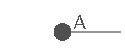
\includegraphics{graphics/concept/operations/CRE} &
  $ \emptyset $ & $ \rightarrow $ & $ A $ & &
  $ \emptyset $ & $ \rightarrow $ & $ A_N $ & &
  $ \emptyset $ & $ \rightarrow $ & $ A_T $ \\

  \midrule
  ICH & Identity Change & 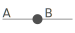
\includegraphics{graphics/concept/operations/ICH} &
  $ A   $ & $ \rightarrow $ & $ B $ & &
  $ A_N $ & $ \rightarrow $ & $ B_N $ & &
  $ A_T $ & $ \rightarrow $ & $ B_T $ \\

  \midrule
  CES & Cessation & 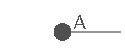
\includegraphics{graphics/concept/operations/CRE} &
  $ \emptyset $ & $ \rightarrow $ & $ A $ & &
  $ \emptyset $ & $ \rightarrow $ & $ A_N $ & &
  $ \emptyset $ & $ \rightarrow $ & $ A_T $ \\

  \midrule
  \multirow{3}{*}{UNI} &
  \multirow{3}{*}{Unification} &
  \multirow{3}{*}{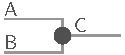
\includegraphics{graphics/concept/operations/UNI}} &
  $ A $ & $ \rightarrow $ & $ C $ & &
  $ A_N $ & $ \rightarrow $ & $ \emptyset $ & &
  $ A_T $ & $ \rightarrow $ & $ \emptyset $ \\
  & & &
  $ B $ & $ \rightarrow $ & $ C $ & &
  $ B_N $ & $ \rightarrow $ & $ \emptyset $ & &
  $ B_T $ & $ \rightarrow $ & $ \emptyset $ \\
  & & &
  & & & &
  $ \emptyset $ & $ \rightarrow $ & $ C_N $ & &
  $ \emptyset $ & $ \rightarrow $ & $ C_T $ \footnotemark \\

  \midrule
  \multirow{2}{*}{INC} &
  \multirow{2}{*}{Incorporation} &
  \multirow{2}{*}{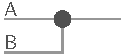
\includegraphics{graphics/concept/operations/INC}} &
  & & & &
  $ (A_N $ & $ \rightarrow $ & $ A_{N'}) $ & &
  $ A_T $ & $ \rightarrow $ & $ A_{T'} $ \footnotemark \\
  & & &
  $ B $ & $ \rightarrow $ & $ A $ & &
  $ B_N $ & $ \rightarrow $ & $ \emptyset $ & &
  $ B_T $ & $ \rightarrow $ & $ \emptyset $ \\

  \midrule
  \multirow{3}{*}{SEP} &
  \multirow{3}{*}{Separation} &
  \multirow{3}{*}{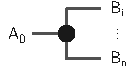
\includegraphics{graphics/concept/operations/SEP}} &
  $ A $ & $ \rightarrow $ & $ B $ & &
  $ A_N $ & $ \rightarrow $ & $ \emptyset $ & &
  $ A_T $ & $ \rightarrow $ & $ \emptyset $ \\
  & & &
  $ A $ & $ \rightarrow $ & $ C $ & &
  $ \emptyset $ & $ \rightarrow $ & $ B_N $ & &
  $ \emptyset $ & $ \rightarrow $ & $ B_T $ \\
  & & &
  & & & &
  $ \emptyset $ & $ \rightarrow $ & $ C_N $ & &
  $ \emptyset $ & $ \rightarrow $ & $ C_T $ \footnotemark \\

  \midrule
  \multirow{2}{*}{SEC} &
  \multirow{2}{*}{Secession} &
  \multirow{2}{*}{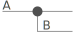
\includegraphics{graphics/concept/operations/SEC}} &
  $ A $ & $ \rightarrow $ & $ B $ & &
  $ (A_N $ & $ \rightarrow $ & $ A_{N'}) $ & &
  $ A_T $ & $ \rightarrow $ & $ A_{T'} $ \\
  & & &
  & & & &
  $ \emptyset $ & $ \rightarrow $ & $ B_N $ & &
  $ \emptyset $ & $ \rightarrow $ & $ B_T $ \footnotemark \\

  \midrule
  \multirow{1}{*}{NCH} &
  \multirow{1}{*}{Name Change} &
  \multirow{1}{*}{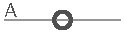
\includegraphics{graphics/concept/operations/NCH_TCH}} &
  & & & &
  $ A_N $ & $ \rightarrow $ & $ A_{N'} $ & &
  & & \\

  \midrule
  \multirow{2}{*}{BCH} &
  \multirow{2}{*}{Border Change} &
  \multirow{2}{*}{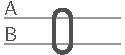
\includegraphics{graphics/concept/operations/BCH}} &
  & & & &
  & & & &
  $ A_T $ & $ \rightarrow $ & $ A_{T'} $ \\
  & & &
  & & & &
  & & & &
  $ B_T $ & $ \rightarrow $ & $ B_{T'} $ \footnotemark \\

  \midrule
  \multirow{1}{*}{TCH} &
  \multirow{1}{*}{Territory Change} &
  \multirow{1}{*}{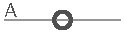
\includegraphics{graphics/concept/operations/NCH_TCH}} &
  & & & &
  & & & &
  $ A_T $ & $ \rightarrow $ & $ A_{T'} $ \\

  \bottomrule
\end{tabular}
\caption{Overview about all 10 historical geographic operations}
\label{tab:historical_geographic_operations}
\end{center}
\end{table}[H]

\addtocounter{footnote}{-4}
\footnotetext{$C_{T} = A_T \cup B_T$}
\addtocounter{footnote}{1}
\footnotetext{$A_{T'} = A_T \cup B_T$}
\addtocounter{footnote}{1}
\footnotetext{$B_T \cup C_{T} = A_T$}
\addtocounter{footnote}{1}
\footnotetext{$A_{T'} \cup B_{T} = A_T$}
\addtocounter{footnote}{1}
\footnotetext{$A_{T} \cup B_{T} = A_{T'} \cup B_{T'}$}

% paragraph historical_geographic_operations (end)

% - - - - - - - - - - - - - - - - - - - - - - - - - - - - - - - - - - - - - - -

combination of cases

There are topological rules rules that can be applied, e.g. two neighboring countries (polygons) share one common border (polyline). That preserves the relationship between them if their common border changes.

MECE principle: Mutually Exclusive and Collectively Exhaustive


A data model is an incomplete abstraction of the real world to develop a reasonable solution for the problem space.
Since the data model uses the concept of several existing one, it will derive also its name from it: The Hivent-Based Three-Domain Spatio-Temporal History Graph Data Model for Time-Stamped Vector Geometry
... or in short: HBTDSTHGDMTSVG

estd for vector graphics

3 domain model
identity: formal name of an entity

history graph model without changing state: active, inactive

simplification: just active / inactive, normal / contested + level of certainty

no transaction time, only valid / event time
only world time is regarded, not database time.


interior borders of countries, which are straight lines between manually defined border points.
=> vector model

A main problem is to maintain the integrity of the spatial topology when a new change gets inserted not at the end of the list. A simple example shows that problem: Given geo-object $X$ is part of the inital base configuration at change $t_b$. At a later change, e.g. $t_y$ $X$ gets replaced by object $Y$. If a new change that updates $X$ to $X'$ gets inserted before at time point $t_x < t_y$, then $t_y$ is not integer anymore, because object $X$ does not exist. That is why on insertion of a change, all succeeding changes have to be tested for integrity and it might be necessary to update later changes.

% \begin{figure}[ht]
%   \centering
%   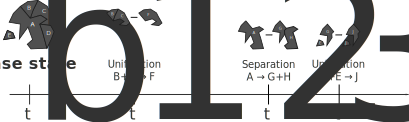
\includegraphics[width=0.8\textwidth]{graphics/basics/stdm/event-based_spatio-temporal_data_model}
%   \caption{The Event-Based Spatio-Temporal Data Model}
%   \label{fig:event-based_spatio-temporal_data_model}


\paragraph{possible extension} % (fold)
\label{par:possible_extension}

% paragraph possible_extension (end)

-> the whole earth is 100\% covered by spatial objects (full topology)
  countries, debated territories, unknown land, water
  Newtons concept of absolute space?


inclusion of universe $\Omega$:
CRE = SEC from $\Omega$
DES = INC into $\Omega$

% subsection historical_changes (end)


% section hivent_model (end)


store Hivents in DoublyLinkedList


% \subsection{Four-Domain Model}
\label{sub:four_domain_model}

According to the extension of the Three Domain model (see section \ref{sub:three_domain_model}), a spatio-temporal object can be represented separetely in the spatial, temporal and thematic domain. Additionally, the semantic domain uniquely identifies an object and is invariant. This applies to the concept of an Area that represents a country.


id: formal name

semantic: id (formal name)
spatial:  spatial attributes (territory)
temporal: Hivent -> HistoricalChange -> AreaChange
thematic: aspatial attributes (short name)

% subsection four_domain_model (end)

% ==============================================================================
\section{HistoGlobe} % (fold)
\label{sec:histoglobe}

Application: HistoGlobe
A distributed \emph{Web Information System}, consists of a remote server side, on which the storage and management of the actual data happens, and the client side on which the user communicates with the system. It hosts the user interface that is rendered in a Web browser.

map for spatial domain (x, y)
timeline for temporal domain (t)
-> 3D system

describe the components of the HG explicitally

ancestors successors
layers of administrative units
open to extension for additional attribute data (e.g. statistics)

requirements
  geographical knowledge
  contextualize / intersect historical sources
  accept imprecision
  prevent illusion of certainty

usable User Interface for both navigation and editing
-> problem: all interfaces are trés horrible!



% ------------------------------------------------------------------------------
\subsection{System Architecture} % (fold)
\label{sub:system_architecture}

The system developed in this thesis is Web-based. That means, there is a \emph{client}, a Web browser, and a remote Web \emph{server} with a database and a middleware. The Web browser hosts the applications user interface. If the user interacts with a tool the client sends a request to the Web server for new data. The middleware checks the request and queries the necessary data from the database. The data will be transformed and sendt back to the client. On the map and the timeline the new information will be shown.

This clear separation between the data (\emph{model}), the user interface (\emph{view}) and the middleware (\emph{controller}) follows directly from the \emph{model-view-controller pattern}: One part can be changed without interfering the other parts, e.g. if the 2D map is replaced by a 3D globe, only the view changes, but the middleware and the database can stay untouched. Likewise, the implementation of a new database technology has no consequences to the view.

% subsection system_architecture (end)


% ------------------------------------------------------------------------------
\subsection{Data Input} % (fold)
\label{sub:input}

This HGIS needs data about historical countries, their names and borders and historical events that lead to historical changes of these countries. There are a lot of free and open sources for geographic data about the current countries, their names and borders. One of the most exhaustive collections of geographic data in public domain is hosted by Natural Earth
\footnote{
  \textit{Natural Earth},
  URL: \url{http://www.naturalearthdata.com/downloads/},
  last access: 30.10.2015
}.
There is physical data (e.g. coastlines, rivers, or glacier areas) and cultural data (e.g. political borders, cities, roads, airports or timezones). OpenStreetMap also opens its database to the public
\footnote{
  \textit{Planet OSM},
  URL: \url{http://planet.openstreetmap.org/},
  last access: 30.10.2015
}.

However, data about historical countries and events are not as straightforward to aquire, because of the mostly qualitative nature of historical research (see section \ref{sub:history}). The most exhaustive free and open source of historical is the \emph{Wikipedia} and their article categories, e.g. \texttt{armistices} or \texttt{treaties}
\footnote{
  \textit{Category:Treaties},
  Wikipedia, the free encyclopedia,\\
  URL: \url{https://en.wikipedia.org/wiki/Category:Treaties},
  last access: 13.05.2016
}.
All sorts of historical events can be found, even translated into different languages. Some information is structured in information boxes, e.g. some historical treaties have a name, an image, a location, a signature and an effect date, an overview about treaty conditions and signatories. Particularily interesting for this thesis are articles about historical countries
\footnote{
  \textit{List of former sovereign states},
  Wikipedia, the free encyclopedia,
  URL: \url{https://en.wikipedia.org/wiki/List_of_former_sovereign_states},
  last access: 13.05.2016
},
because they contain the name of the country and meta information, e.g. their historical successors and predecessors. Building an open-source Historical Geographic Information System on the basis of Wikipedia would be a huge project with significant impact on the world of free and open education --- however, it would also be a big challenge: Wikipedia is incomplete, not all historical countries and events necessary to model the history of the world are available. It is also inconsistent, because not all articles about historical countries and events are structured, especially not to those who actually have an influence on a territorial change of a country, e.g. a border agreement. Retrieving, parsing and processing this information is a big challenge. Also the problem of accuracy and quality of information in the Wikipedia due to their open source nature has to be considered. Overall, using the Wikipedia as a data source for this thesis is not feasible, but is subject to further research.

% - - - - - - - - - - - - - - - - - - - - - - - - - - - - - - - - - - - - - - -
\paragraph{Historical maps} % (fold)
\label{par:historical_map}

The most problematic data to acquire is about the territories and borders of historical countries. There is no primary data source for that, so the only way to retrieve a border is to extract it from an historical map.

They also can be found on Wikipedia, or in historical map colletions, e.g. \emph{OldMapsOnline}. The project is developed ``out of a love of history and heritage of old maps'' and currently stores about 400000 historical maps
\footnote{
  \textit{Old Maps Online},
  URL: \url{http://www.oldmapsonline.org/},
  last access: 13.05.2016
}.
There are five steps to retrieve a border with points in geographic coordinates from an historical map.
\begin{enumerate}
  \item \textbf{Digitization}: If the map is on paper, it has to be scanned in the best possible quality. The result is a raster graphic.
  \item \textbf{Georeferencing}: The historical map has to fit as good possible on the reference map. This requires to manually define a set of reference points which are used to transform the map into the geographic coordinate system. This process is error-prone, especially if the projection of the historical map is not known and the map itself is not accurate
  \cite[pp. xvii]{knowles2002past}.
  The outcome is a raster graphic in which each pixel is assigned a geographic coordinate.
  \item \textbf{Preprocessing}: The raster image has to be be processed so that the desired border stands out and can be traced in the next step. This happens via greyscale conversion, thresholding or the Canny Edge Detector. This results in a monochrome graphic in which the desired border must be uninterrupted and clearly be seen.
  \item \textbf{Line detection}: By selecting a start and an end point of the border, the line gets traced automatically. This step vectorizes one particular feature, a borderline, from the raster graphic and produces a polyline in geographic coordinates.
  \item \textbf{Postprocessing}: In the last step, the polyline can be adapted: The line can be simplified to reduce unnatural artifacts and the position of border points can be manually edited. The final output of the whole process is a polyline whose points are expressed in the geographic coordinate system which can be used in the system as a border of an historic country.
\end{enumerate}

This process was developed in a preceding \emph{HiBo} project
\footnotetext{
  \textit{HiBo - semi-automatic extraction of borders from historical maps},
  Project of: B. Weber, N. K. Dankwa, K. Singh and T. Kashyappan, supervised by: Prof. Volker Rodehorst and Marcus Kossatz, Bauhaus-Universität Weimar, February 2015,
  URL: \url{https://bitbucket.org/bastian_weber/hibo},
  last access: 29.10.2015
}
(see figure \ref{fig:hibo}).

\begin{figure}[ht]
  \centering
  \begin{subfigure}{0.48\textwidth}
    \centering
    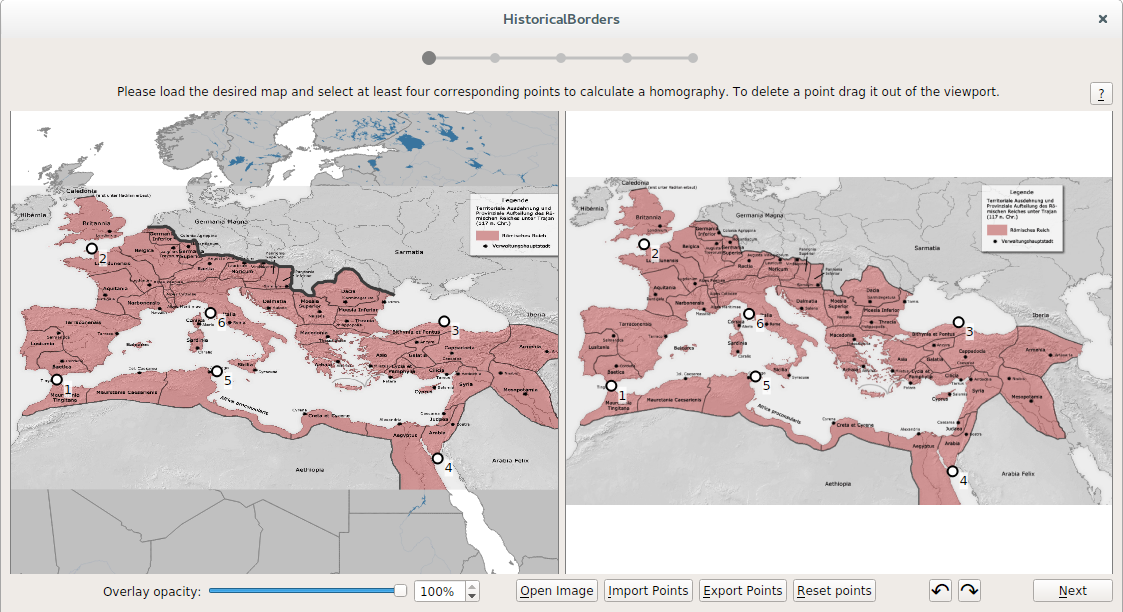
\includegraphics[width=0.95\linewidth]{graphics/basics/hibo1.png}
    \caption{Georeferencing}
  \end{subfigure}
  \begin{subfigure}{0.48\textwidth}
    \centering
    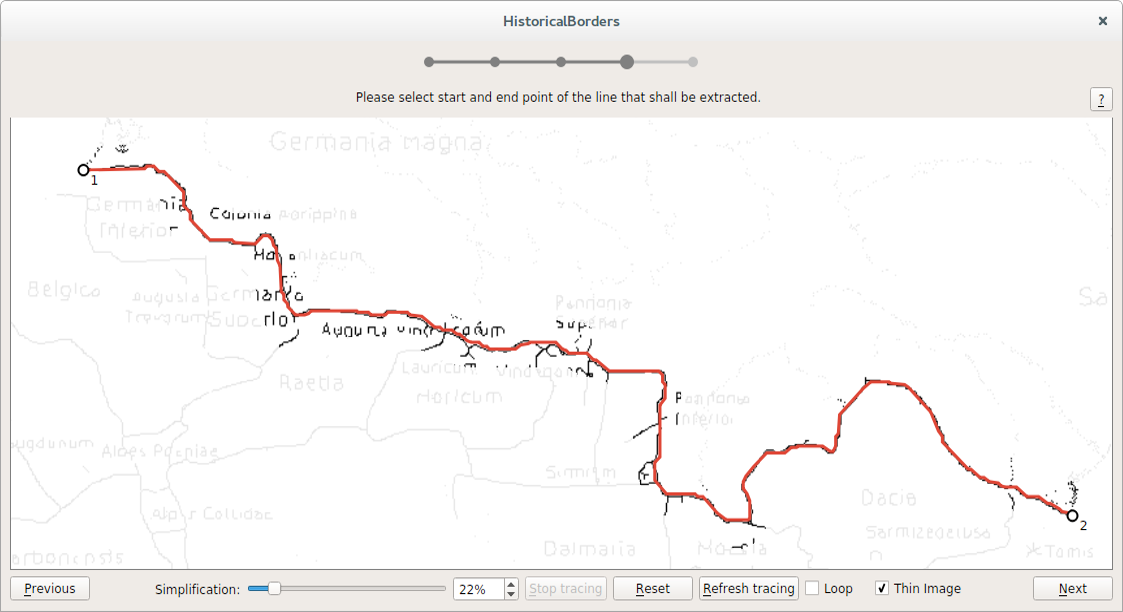
\includegraphics[width=0.95\linewidth]{graphics/basics/hibo2.png}
    \caption{Semi-automatic digitizing}
  \end{subfigure}
  \caption{Semi-automatic extraction of a border from a map of the Roman Empire \protect\footnotemark}
  \label{fig:hibo}
\end{figure}

% paragraph historical_map (end)


% - - - - - - - - - - - - - - - - - - - - - - - - - - - - - - - - - - - - - - -
\paragraph{Manual data input} % (fold)
\label{par:manual_data_input}

For the domain of this HGIS, the development of countries over time, there is no complete dataset available. Therefore, the system developed in this thesis needs to have an interface to enter historical data. The user needs to have an interface to enter information about historical events that change territories and names of historical countries. This data has to be acuired either from primary historical sources directly, or from free online sources. Next to Wikipedia, there are other collections of historical events, e.g. \emph{Correlates of War}
\footnote{
  \textit{Data Sets},
  Correlates of War,
  URL: \url{http://www.correlatesofwar.org/data-sets/folder_listing},
  last access: 13.05.2016
}
for quantitative data about international relations.
% paragraph manual_data_input (end)

% subsection data_input (end)



% ------------------------------------------------------------------------------
\subsection{Edit Mode} % (fold)
\label{sub:edit_mode}


user operations     CRE     UNI          SEP         TCH         NCH      DES
                     |      / \         /   \        /  \       /   \      |
HG operations       CRE   UNI   INC   SEP   SEC   TCH   BCH   NCH   ICH   DES

area changes        ADD   DEL*  DEL*  DEL   TCH   TCH   TCH   NCH   ADD   DEL
ADD, TCH, NCH, DES        ADD   TCH   ADD*  NCH?        TCH         DEL
                                NCH?        ADD*


geometries must be edited



% subsection edit_mode (end)

% ------------------------------------------------------------------------------
\subsection{HistoGraph} % (fold)
\label{sub:histograph}

% subsection histograph (end)

% section histoglobe (end)



% chapter concept (end)
%!TEX root = ../thesis.tex

\section{Development} % (fold)
\label{sec:development}


% ==============================================================================
\subsection{System Architecture} % (fold)
\label{sub:system_architecture}

% subsection system_architecture (end)


% ==============================================================================
\subsection{Interface Design} % (fold)
\label{sub:interface_design}

% subsection interface_design (end)


% ==============================================================================
\subsection{Client-Side Application} % (fold)
\label{sub:client_side_application}

% subsection client_side_application (end)


% ==============================================================================
\subsection{Server-Side Application} % (fold)
\label{sub:server_side_application}

view

models

% subsection server_side_application (end)



% ==============================================================================

% section development (end)
%!TEX root = ../masters_thesis.tex

\section{Uncertainty} % (fold)
\label{sec:uncertainty}

Every aspect of the concept (section \ref{sec:concept}) and the development (section \ref{sec:development}) of this work is based on the prerequisite of full certainty of the data. That means both the Historical-Geographic Operations and the Hivent-Based Spatio-Temporal Data Model assume that the dates of the historical events, the names and territories of the historical and current areas and the historical relations between events and areas are correct, accurate, exact and precise (definitions see \ref{sub:types_of_uncertainty}).

However, this assumption is far from valid. In historical research, uncertainty is one of the major problems (see \ref{ssub:history}) a historian has to deal with on a daily basis: sources, even primary sources, can be biased towards the author of the source, information can be imprecise or inaccurate and information can be conflicting with other sources. The purpose of this section is to introduce the problem of uncertainty in the domain of this thesis, explain the main concepts and develop solutions to deal with this problem.


% ==============================================================================
\subsection{Definition of a Country} % (fold)
\label{sub:definition_of_a_country}

The problem begins with the definition of a term that almost everybody in the world is familiar with: a ``country''. But the search for a non-conflicting explanation of what a country actually is leads to a dead end.

The Oxford Dictionary definition includes the human and the territorial aspect of a country: ``An area of land of defined extent characterized by its \emph{human occupants} or \emph{boundaries}.''
\footnote{\textit{country, n. and adj}, Oxford English Dictionary, URL: \url{http://www.oed.com/view/Entry/43085?}, last access: 2016-04-25}

The CIA Factbook collects, manages and visualizes data and facts ``on every country, dependency, and geographic entity in the world''. Its definition of a country should therefore be helpful to understand what a country actually is. In the database the term \emph{political entity} is defined like this: An ``Independent state refers to a people politically organized into a sovereign state with a \emph{definite territory}. \emph{Dependencies} and \emph{areas of special sovereignty} refer to a broad category of political entities that are associated in some way with an independent state.''
\footnote{\textit{The World Factbook}, CIA Factbook, URL: \url{https://www.cia.gov/library/publications/the-world-factbook/docs/notesanddefs.html\#T}, last access: 2016-04-25}

The CIA Factbook includes a total of 267 ``separate geographic entities'' in five different categories:
\begin{enumerate}
  \item 195 independent states (e.g. Germany, the United Kingdom or Swaziland)
  \item 2 ``other'' states (Taiwan and the European Union),
  \item 85 ``dependencies and areas of special sovereignty'' (e.g. Greenland to Denmark, Hong Kong to China or Puerto Rico to the United States),
  \item 6 ``miscellaneous'' entities (Antarctica, the Gaza Strip, Paracel Islands, Spratly Islands, West Bank, Western Sahara) and
  \item 5 ``other entitites'' (Arctic, Atlantic, Indian, Pacific and Southern Ocean)
\end{enumerate}

Excluding other entities, there are four different groups of political entities used in the Factbook. While Antarctica as an uninhabitated place might not be a surprising miscellaneous entity, the Gaza Strip and the West Bank as the two territories associated to Palestine, Taiwan, Hong Kong or Greenland are not listed as independent states

The most importatn source for countries in the world is probably the United Nationals. The intergovernmental organisation was found after World War II (October 1945) and promotes international peace keeping, security, protection of human rights or humanitarian aid. The committee has 193 full member states
\footnote{\textit{Member States}, United Nations, URL: \url{http://www.un.org/en/member-states/index.html}, last access: 2016-04-25}
and two permanent obervers: The Holy See (Vatican City) and Palestine.
\footnote{\textit{Non-member States}, United Nations, URL: \url{http://www.un.org/en/sections/member-states/non-member-states/index.html}, last access: 2016-04-25}.

The two lists yield some interesting observations:
\begin{enumerate}
  \item The Holy See is the juridcal and spiritual entity representing the territory of Vatican City. It is classified as an independent state by the CIA but is not a full member of the UN, because it has never applied for it. However, it is a fully sovereign country with diplomatic relations to the vast majority of countries in the world -- which makes it the by far smallest sovereign state in the world (0.44 m²), inside the city of Rome with a population of only 800 people, including 30 women.\footnote{\textit{Population}, Vatican City State, URL: \url{http://www.vaticanstate.va/content/vaticanstate/en/stato-e-governo/note-generali/popolazione.html}, last access: 2016-04-25}

  \item The State of Palestine, consisting of the territories of the West Bank and the Gaza Strip and a population of 4.4 million people,\footnote{\textit{Estimated Population in the Palestinian Territory}, Palestinian Central Bureau of Statistics, URL: \url{http://www.pcbs.gov.ps/Portals/_Rainbow/Documents/gover_e.htm}, last access: 2016-04-25}
  has the same status in the United Nations (observer state), but a totally different situation in terms of sovereignty: First of all, it does not have a clearly defined territory. Additionally, while 114 states officially recognize the Palestinian state, almost all main economic powers do not, including the United States, Canada, France, Italy, Germany or the United Kingdom. None of them even voted in favor of Palestine receiving an observing status in the UN.\footnote{\textit{General Assembly Votes Overwhelmingly to Accord Palestine ‘Non-Member Observer State’ Status in United Nations}, United Nationals, URL: \url{http://www.un.org/press/en/2012/ga11317.doc.htm}, last access: 2016-04-25}
  That means, unlike the Holy See, Palestine is not a fully sovereign and recognized state.

  \item Kosovo is listed by the CIA Factbook as an independend nation, after having seceded from Serbia and declared independence in 2008. It has a clearly defined territory and population and is recognized by 111 UN member states. However, among the five permanent members of the United Nations Security Council (USA, UK, France, Russia and China), the latter two veto the membership of Kosovo in the United Nations -- but UN membership requires full approval by all members of the security council. Therefore, Kosovo is not even an observer state of the United Nations, although having about the same degree of international recognition as Palestine.
  \footnote{\textit{Who Recognizes Kosova?}, URL: \url{http://www.kosovothanksyou.com}, last access: 2016-04-25}

  \item The status of Taiwan is a very complicated issue. An overgeneralized and short description of the problem, in which two territories and two political entities are involved in, is: There is the People's Republic as China (commonly known as China) with full control over mainland China and the Republic of China, governing the island of Taiwan. However, both political entities claim each others land. That means, there are two entities claiming the exact same land. But, since 1971 the People's Republic of China is the representative of whole China in the United Nations, including the island of Taiwan. Since it is part of the Security Council, it successfully vetos membership requests of Taiwan. Therefore, the Republic of China can not be a member of the United Nations. Currently, 22 member states of the United Nations uphold official diplomatic relations to Taiwan.\footnote{\textit{Ministry of Foreign Affairs}, Republic of China, URL: \url{http://www.mofa.gov.tw/en/default.html}, last access: 2016-04-25}
  All of these states do not have any diplomatic relations to the People's Republic of China which makes it an only partially recognized state.

\end{enumerate}

In Addition to these special cases, there are five other member states of the United Nations that are not fully recognized by all other UN members: Armenia (not recognized by Pakistan), the Republic of Cyprus (not recognized by Turkey), North and South Korea (officially Democratic People's Republic of Korea and Republic of Korea, mutual non-recognition) and the State of Israel, which 32 UN member states do not recognize.

Finally, there are non-member states of the United Nations which have not yet gained broad international recognition: the Sahrawi Arab Democratic Republic (recognized by 84 UN member states), Abkhazia (6), South Ossetia (5), the Turkish Republic of Northern Cyprus (1) Nagorno-Karabakh Republic (0), Transnistria (0) and Somaliland (0).
\footnote{\textit{List of states with limited recognition}, Wikipedia, URL: \url{https://en.wikipedia.org/wiki/List_of_states_with_limited_recognition}, last access: 2016-04-25}

Everything breaks down to the problem of the definition of a country, which is based on two concepts: The \emph{declarative theory} and the \emph{constituitive theory}:


% ------------------------------------------------------------------------------
\subsection{Declarative Theory} % (fold)
\label{sub:declarative_theory}

Montevideo Convention
=> Area
% subsection declarative_theory (end)

% ------------------------------------------------------------------------------
\subsection{Constituitive Theory} % (fold)
\label{sub:constituitive_theory}


=> status
% subsection constituitive_theory (end)

% ------------------------------------------------------------------------------

-> problem: self-classifying and conflicting entities / data => impossible to create data model that fits everything
=> have to develpo approaches and know that it is wrong

% subsection definition_of_a_country (end)


% ==============================================================================
\subsection{Types of Uncertainty} % (fold)
\label{sub:types_of_uncertainty}

accuracy vs. precision
correctness vs. exactness

uncertainty vs. different stories

historical      when?       -> unclear sources, different sources, different calendars, timezones
geographic      where?      -> unclear sources (historical maps), contestes borders / territories
information     what? how?  -> unclear sources, different names, different viewpoints
system          why?        -> very subjective, very uncertain


% subsection types_of_uncertainty (end)



% ==============================================================================
\subsection{Fuzzy Systems} % (fold)
\label{sub:fuzzy_systems}

problem: uncertainty

% subsection fuzzy_systems (end)


% ==============================================================================
\subsection{Solution Approaches} % (fold)
\label{sub:solution_approaches}

% subsection solution_approaches (end)


% ==============================================================================

% section uncertainty (end)
%!TEX root = ../masters_thesis.tex

\chapter{Summary} % (fold)
\label{cha:summary}
has a great potential to teach, learn and understand processes in the past. A system that is able to tell \emph{what} happened and \emph{where} the historical event has influences on and \emph{when} the event happened happened might be tool to answer the most important of all questions:
\textbf{\emph{Why}} it happened?


finally to reason about if wars actually make sense.
If John Lennon is right, then this HGIS has come to its ultimate end: all Areas have unified. All the people living life in peace. You may say I am dreamer, but I am not the only. I hope someday you'll join us. And the world will be as one.

% ==============================================================================
\section{Results} % (fold)
\label{sec:results}

% section results (end)


\paragraph{Research Questions} % (fold)
\label{par:result_research_questions}

% paragraph result_research_questions (end)


% ==============================================================================
\section{Problems} % (fold)
\label{sec:problems}

% section problems (end)



% ==============================================================================
\section{Future Work} % (fold)
\label{sec:future_work}

step further: temporal GIS to narrative GIS

idea: explain history with spatial narratives
  geographically contextualize events and interactions
  organizing principle: time

extend the pure presentational purpose of st data to analytical purpose, e.g. where have most border changes take place in previous 200 years?

Another problem for historians is that they do not necessarily need a tool to better visualize existing knowledge (e.g. historical maps), but to generate new knowledge by analyzing spatio-temporal coherences or distributions in historical data. Spatio-temporal reasoning is still an open field and not easily possible with existing HGIS

\cite[p. 268]{knowles2008placing}, \cite[p. xii]{gregory2014toward}.
space-time premise by Gaddis 2002
  time and space equal importance
  event     what significantly has happend and by whom? (singularity!)
  process   how something has happened? (event+activity => trigger of process)
  change    driven by process
  spatiotemporal data defines all above three
  % \cite Gaddis 2002

extend area model to hierachies (country -> states -> counties/cities)

% section future_work (end)


% ==============================================================================

% chapter summary (end)


%\* BIBLIOGRAPHY*\

\bibliography{chapter/x-sources}{}
\bibliographystyle{chapter/alphaurl}


%\* APPENDIX *\

%!TEX root = ../thesis.tex

\section*{Stuff} % (fold)
\label{sec:stuff}

% section stuff (end)



\end{document}
